In analogy to classical mechanics, we can study the quantum system in phase space. In doing so, we arrive to the so-called quasiprobability density functions, which are equivalent to the quantum state and provides yet another operational approach to its characterisation. Unsurprisingly, such analogy finds frontiers, since such quasiprobability distributions can take negative values (for instance, for non-Gaussian states). In this regard, we find that the set of quantum Gaussian states behave classically, since their associated quasiprobabilities are --- spoiler alert --- Gaussian distributions.

The phase-space formalism hinges on the overcompleteness of Weyl operators, which serves as a bridge between Hilbert and phase spaces. In the following we will restrict to the \textit{single}-mode case; generalizations to $n$-mode systems are straightforward.

Recall that a coherent state is defined an eigenstate of $\hat{a}$
\eq{def_coherent}{\begin{cases} \hat{a} \weyl{\alpha} \ket{0} = \alpha \weyl{\alpha}\ket{0} \\ \ket{\alpha} = \weyl{\alpha} \ket{0} \end{cases}.}
In particular, note that $\proj{\alpha} = \weyl{\alpha}\proj{0}\weyl{\alpha}^\dagger$, meaning that coherent states are --- in line with the formalism revisted in the provious section --- just displaced vacuum states, with idle symplectic transformations and thus an identity as covariance matrix. In particular, by writing such states in the Fock basis, we obtain
\eq{1fockcoherent}{\ket{\alpha} = e^{-\frac{|\alpha|^2}{2}} \sum_{n=0}^\infty \frac{\alpha^n}{\sqrt{n}}\ket{n},}from which it is not hard to prove that coherent states resolve to identity:
\eq{resocoh}{\frac{\int_\mathbb{C} \proj{\alpha} d^2\alpha}{\pi} = \id.}
This shows that coherent states resolve to a measurement, called \textit{heterodyne} measurement. Moreover, given any (bounded) operator $\hat{O}$, we can express it as
\begin{align}\label{eq:trW}
\hat{O} &= \frac{1}{\pi} \int_{\mathbb{C}}d^2\alpha \tr{\hat{O} \weyl{\alpha} }\weyl{-\alpha},\\
\tr{\hat{O}} &= \frac{1}{\pi}\int_\mathbb{C} d^2\alpha \langle\alpha|\hat{O}|\alpha\rangle,
\end{align}
which is known as the \textit{Fourier-Weyl relation}. This allows us to write any quantum state $\rho$ in terms of coherent states as
\equ{\rho = \frac{1}{\pi} \int_{\mathbb{C}} \tr{ \rho \weyl{\alpha}} \weyl{-\alpha}.} In particular, the \textit{characteristic function} $\chi(\alpha)$ is defined as the coefficient accompaying $\weyl{-\alpha}$ in the integral, \text{e.g.}
\begin{align}
\chi(\alpha) &= \tr{ \rho \weyl{\alpha}}\\
\rho &= \frac{1}{\pi} \int_{\mathbb{C}} \chi(\alpha)\weyl{-\alpha}.
\end{align}
Such characteristic function allows us to define% quasiprobability distributions, according to
% \eq{qpd}{W_s(\alpha) = \frac{1}{\pi^2} \int_{\mathbb{C}} d^2 \beta \chi_s(\beta) e^{\alpha \bar{\beta} - \bar{\alpha} \beta}}, where it can be checked that $\int W_s(\alpha) d^2 \alpha = 1$.
% Moreover,
the Wigner function as its (complex) Fourier transform:
\eq{qpd}{W(\alpha) = \frac{1}{\pi^2} \int_{\mathbb{C}} d^2 \beta \chi(\beta) e^{\alpha \bar{\beta} - \bar{\alpha} \beta},}
which satisfies that $\int W(\alpha) d^2 \alpha = 1$. By expanding $\alpha = \frac{q + \ii p}{\sqrt{2}} $ and $ \beta = \frac{\tilde{q} + \ii \tilde{p}}{\sqrt{2}}$, we find that $W(q,p) = \int d\tilde{q} e^{\ii p \tilde{q}} \langle q + \tilde{q}| \rho | q - \tilde{q}\rangle$.
Such parametrization provides an operational interpretation of Wigner functions, since $\frac{1}{2}\int_\infty^\infty dp W(q,p)= \langle q |\rho |q\rangle$, \textit{e.g.} marginal distributions predict probability measurement outcomes over conjugate variables and if varying the direction of $p$ in the integrand one can perform a tomographic reconstruction of the quantum state.
\begin{figure}[t!]
\centering
    \begin{subfigure}[b]{0.49\textwidth}
        \centering
        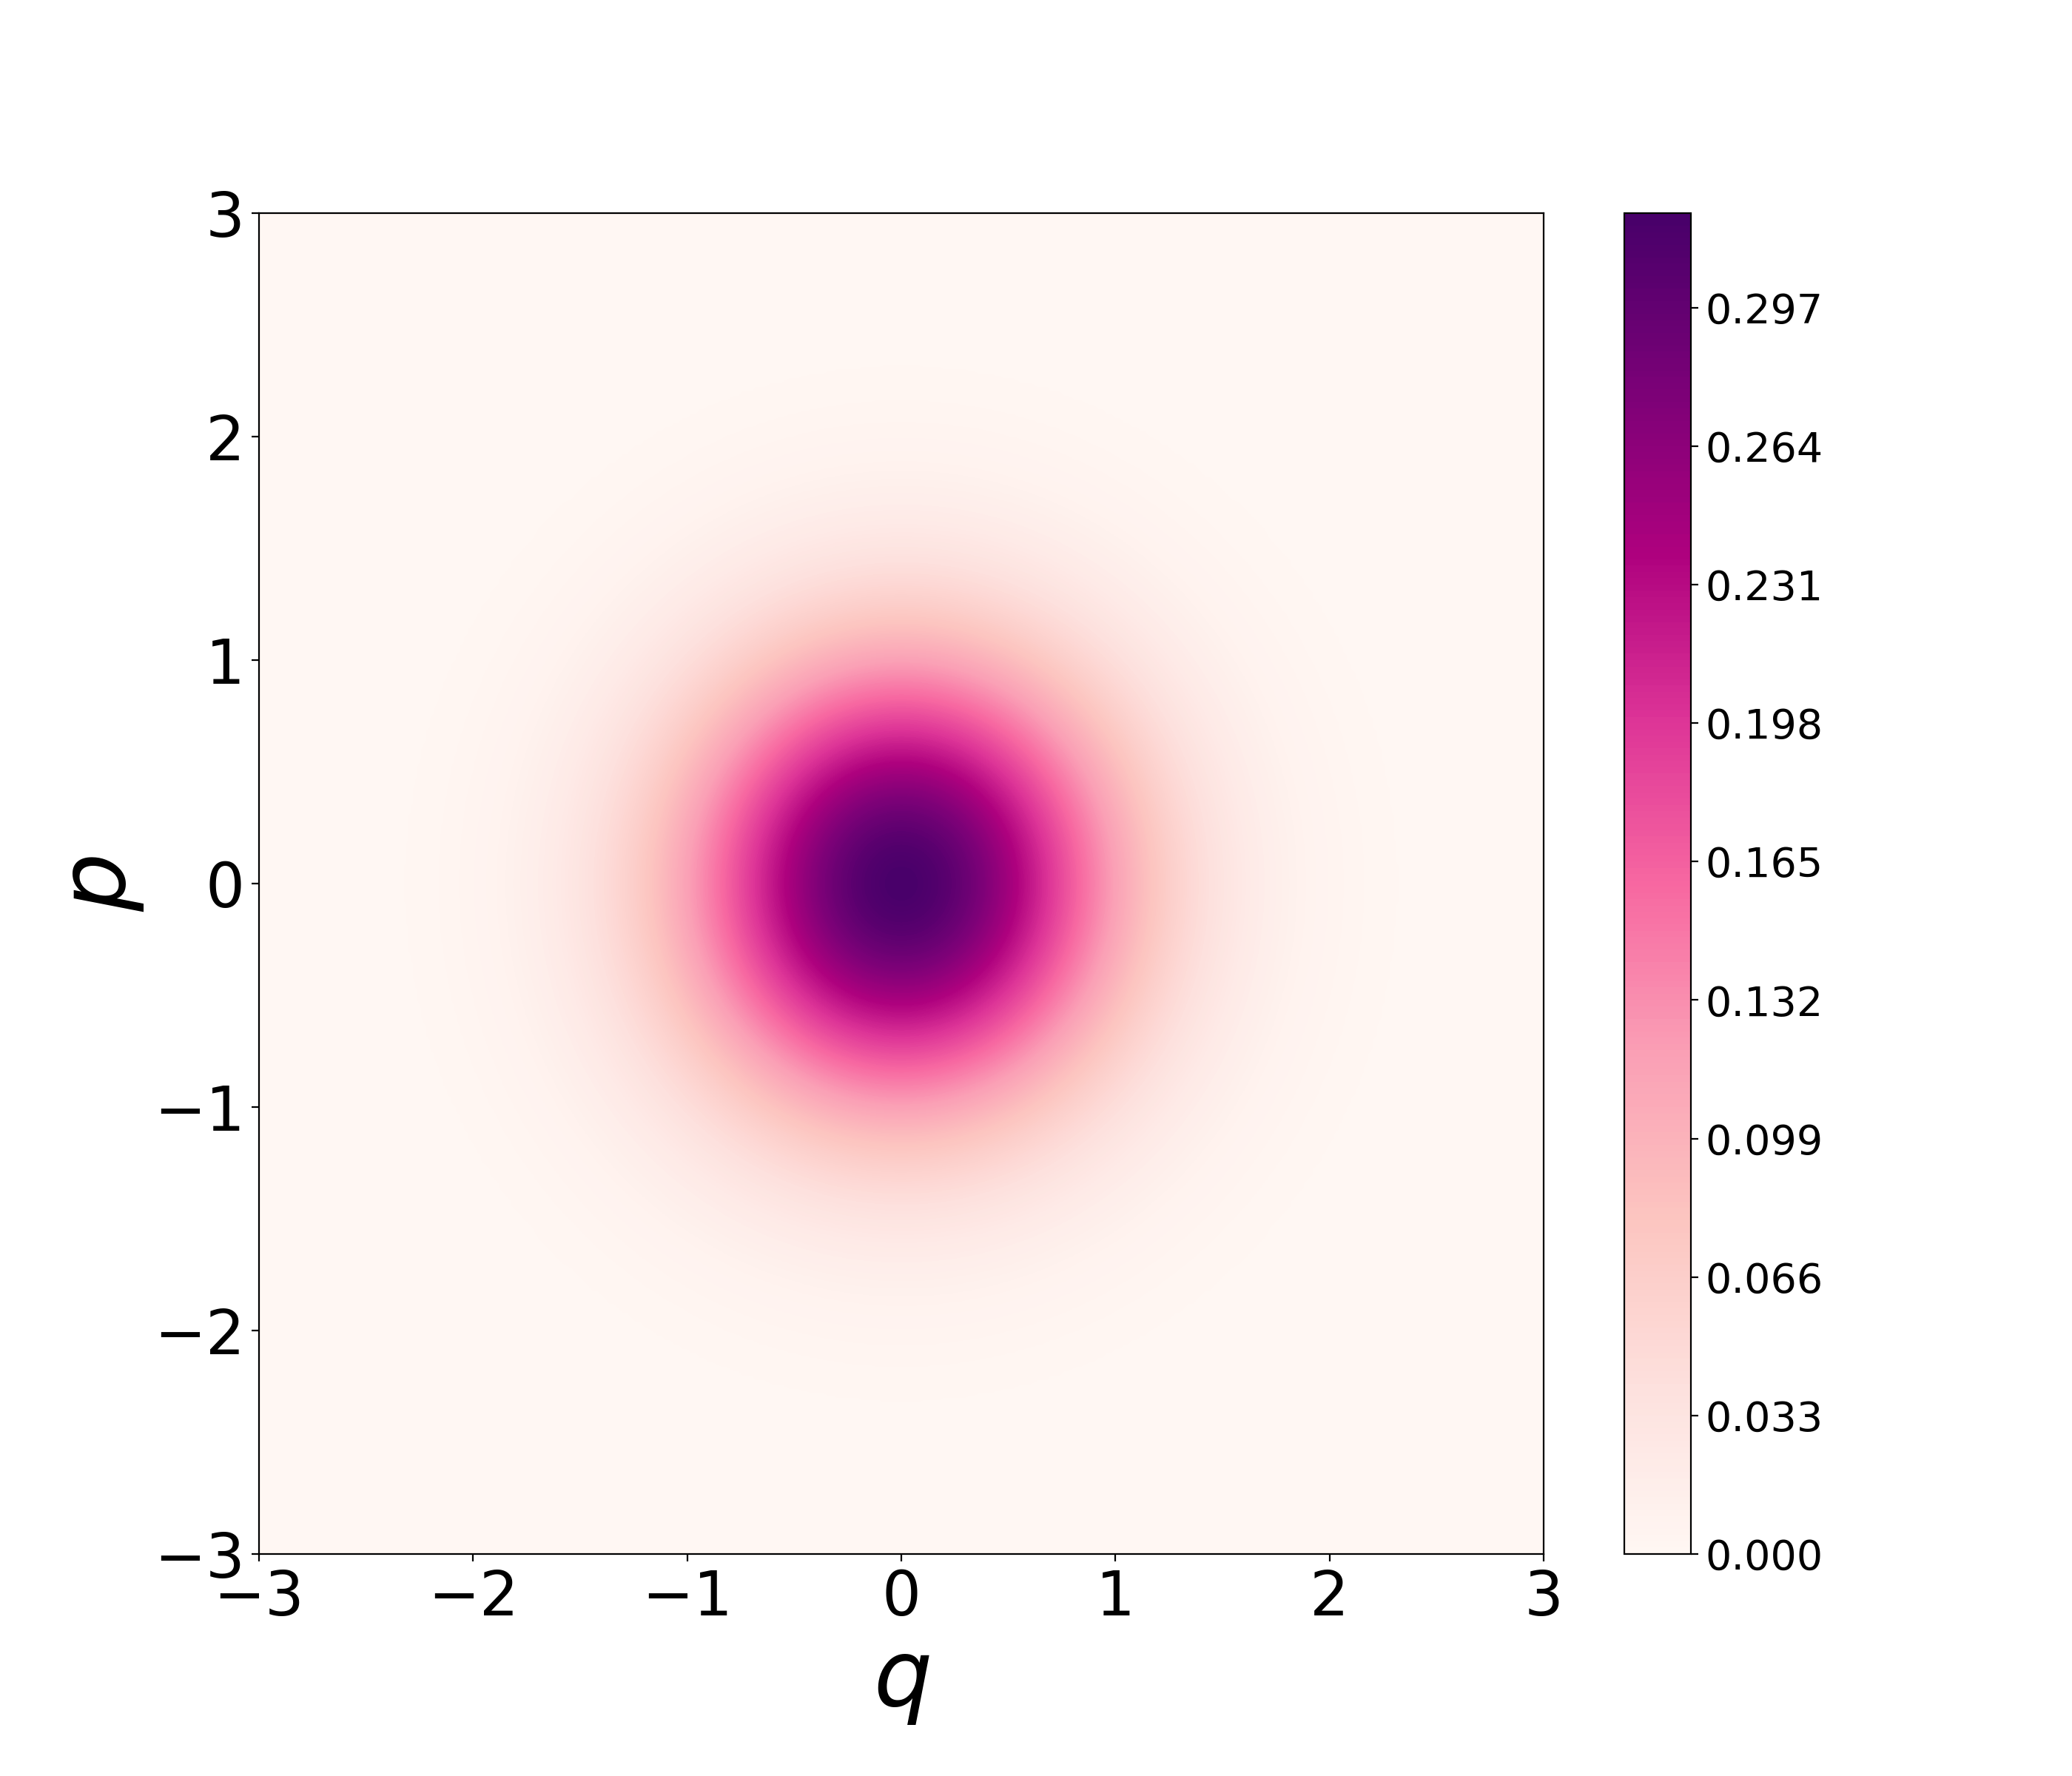
\includegraphics[width=1.\textwidth]{Figures/some_wigners/vacuum.png}
    \end{subfigure}
    \hfill
    \begin{subfigure}[b]{0.49\textwidth}
        \centering
        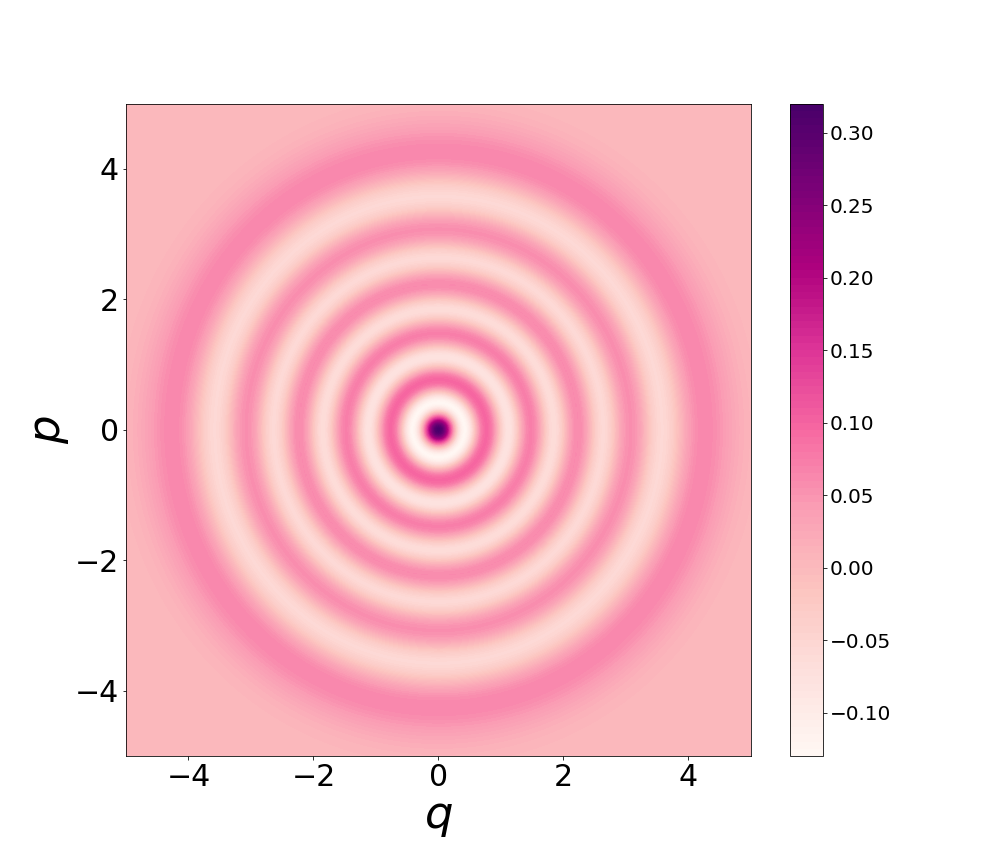
\includegraphics[width=1.\textwidth]{Figures/some_wigners/fock5.png}
    \end{subfigure}
\caption{We show the Wigner functions of the vacuum state $\ket{0}$ (left) and of the Fock state $\ket{5}$ (right). While in the former case the probability distribution is a Gaussian, the latter represents a non-Gaussian state (\textit{e.g.} is the fifth eigenstate of the harmonic oscillator), which here translates into negative values of the Wigner function. }
\label{fig:wigners}
\end{figure}
Finally, for Gaussian states, the characteristic and Wigner functions are Gaussians, \textit{e.g.}
\begin{align}\label{gauss_char_wigner}
\chi(\rvec) &= e^{-\frac{(\Omega \rvec)^T\cov \Omega \rvec}{2} - \ii (\Omega \rvec)^T \bar{\bm{r}}} \\
W(\rvec) &= \frac{2^n}{\pi^n \sqrt{|\cov|}}e^{-(\rvec - \bar{\bm{r}})^T\cov^{-1}(\rvec - \bar{\bm{r}})}.
\end{align}
In Fig.~\ref{fig:wigners} we show two examples of such Wigner functions, one for a coherent (and thus Gaussian) state, and other one for a Fock number state; we observe in the latter case that the Wigner function can take negative values: such negativity play a role of a classical-quantum frontier in continuous-variable systems~\cite{nongaussian}.

We have thus identified the set of Gaussian states as thermal (and ground) states of quadratic hamiltonians. Equivalently, Gaussian states can be defined as those whose characteristic function is Gaussian. On the one hand, we have observed that Gaussian states can be understood as a set of $n$ non-interacting harmonic oscillators, up to a symplectic transformation $\sh$. Such symplectic transformation is ultimately linked to a Gaussian unitary, \textit{e.g.} generated by a quadratic hamiltonian. Moreover, Eq.~\ref{eq:1moms} explicits the action of such transformations on the first two statisitcal moments of the Gaussian state, namely displacing the canonical coordinates and transforming the covariance matrix via a simplectic matrix that acts by similarity. In turn, such operations act linearly in phase space and that is the reason for which Gaussian operations are deemed so in literature~\cite{Weedbrook2012Gaussian,Olivares2012}.
